\chapter{Structure and Design}

\epigraph{In general, when modeling phenomena in science and
  engineering, we begin with simplified, incomplete models. As we
  examine things in greater detail, these simple models become
  inadequate and must be replaced by more refined
  models.}{\textit{Structure and Interpretation of Computer Programs,
    Section 1.1.5}\cite{sicp}}

\section{Structure of combox}


\begin{figure}[h]
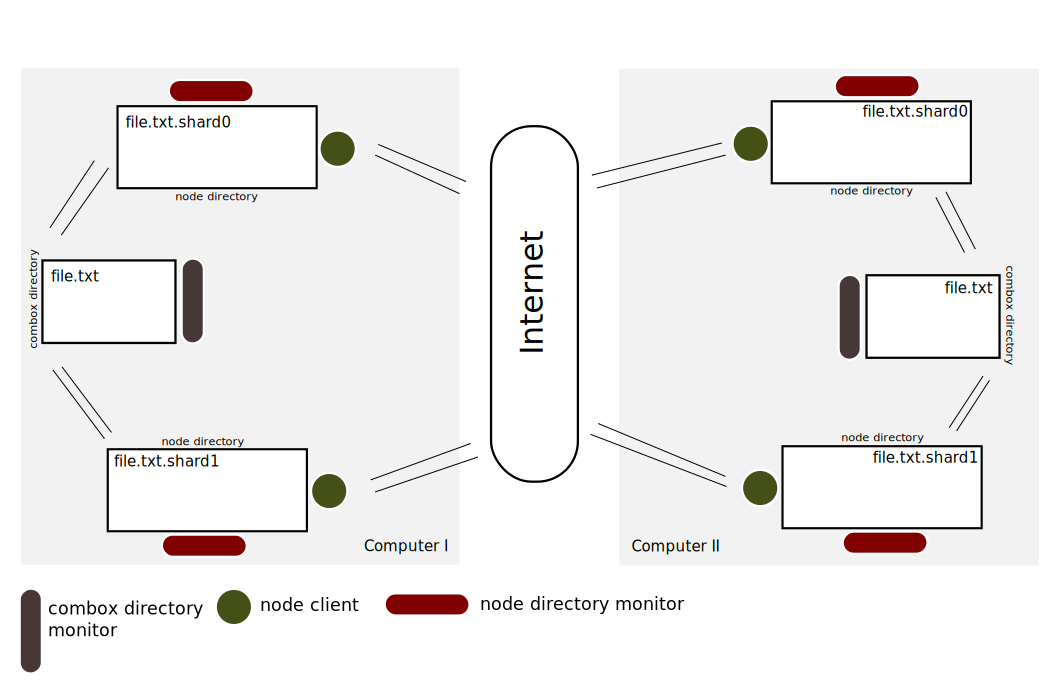
\includegraphics[scale=0.6]{4-combox-structure}
\caption{High level view of combox on two computers.}
\label{fig:4-combox-structure}
\end{figure}

\subsection{combox configuration}

\subsection{combox directory monitor}

\subsection{Node directory monitor}

\subsection{Database structure}

\section{combox modules overview}

\section{Language choice and DRY}

\section{Operating system compatibility}

\section{combox as a python package}

\section{With the benefit of hindsight}